\documentclass[11pt]{article}
\usepackage[a4paper,margin=1in]{geometry}
\usepackage{amsmath,amssymb}
\usepackage[T1]{fontenc}
\usepackage{lmodern}
\usepackage{microtype}
\usepackage{xcolor}
\usepackage{footnote}
\usepackage{tikz}
\usetikzlibrary{arrows.meta,calc}

\setlength{\parindent}{0pt}
\setlength{\parskip}{0.5em}

\newcommand{\promptbox}[1]{%
  \begin{savenotes}%
  \begingroup\setlength{\fboxsep}{10pt}\noindent
  \colorbox{blue!8}{\parbox{\dimexpr\linewidth-2\fboxsep\relax}{\textbf{Prompt. }#1}}
  \endgroup
  \end{savenotes}%
}
\newcommand{\resultbox}[1]{%
  \begin{savenotes}%
  \begingroup\setlength{\fboxsep}{10pt}\noindent
  \colorbox{purple!8}{\parbox{\dimexpr\linewidth-2\fboxsep\relax}{\textbf{Result. }#1}}
  \endgroup
  \end{savenotes}%
}
\newcommand{\examplebox}[1]{%
  \begin{savenotes}%
  \begingroup\setlength{\fboxsep}{10pt}\noindent
  \colorbox{green!8}{\parbox{\dimexpr\linewidth-2\fboxsep\relax}{\textbf{Example. }#1}}
  \endgroup
  \end{savenotes}%
}

\title{\textbf{Book 1 --- Lecture 2 --- Exercise 7}\\[2mm]
\large Orthogonality of Velocity and Acceleration in Uniform Circular Motion}
\author{}
\date{}

\begin{document}
\maketitle

\promptbox{Show that the velocity and acceleration component patterns
\begin{align*}
v_x &= -R\,\omega\sin(\omega t), &
v_y &= R\,\omega\cos(\omega t),\\
a_x &= -R\,\omega^2\cos(\omega t), &
a_y &= -R\,\omega^2\sin(\omega t)
\end{align*}
are orthogonal.\footnote{These are the standard components of \(\mathbf{v}\) and
\(\mathbf{a}\) for uniform circular motion with radius \(R>0\) and angular
frequency \(\omega\) (radians per unit time). Some editions of the notes
misprint the heading as ``position and velocity'' instead of ``velocity and
acceleration''; the algebra below matches the latter. The word
\emph{acceleration} is sometimes mistyped in informal copies (e.g.\
``accelelration''). \(\omega\) is spelled here (not ``omege'').}}

\section*{Vectors}
Write \(\mathbf{v}=(v_x,v_y)\) and \(\mathbf{a}=(a_x,a_y)\). Orthogonality means
\(\mathbf{v}\cdot\mathbf{a}=0\).\footnote{Dot product and orthogonality are
reviewed in Book~1, Lecture~1, Interlude~1, Exercise~6.}

\section*{Dot product}
Multiply termwise and add:
\begin{align*}
\mathbf{v}\cdot\mathbf{a}
&=(-R\omega\sin(\omega t))\bigl(-R\omega^2\cos(\omega t)\bigr)
+\bigl(R\omega\cos(\omega t)\bigr)\bigl(-R\omega^2\sin(\omega t)\bigr)\\
&=R^2\omega^3\sin(\omega t)\cos(\omega t)-R^2\omega^3\cos(\omega t)\sin(\omega t)\\
&=0.
\end{align*}
Hence \(\mathbf{v}\perp\mathbf{a}\) for all \(t\) (and all real \(\omega\), with
the convention that the zero vector is orthogonal to every vector).

\section*{Related orthogonality (position and velocity)}
For the same motion, \(\mathbf{r}(t)=R\bigl(\cos(\omega t),\,\sin(\omega t)\bigr)\)
has derivative \(\mathbf{r}'=\mathbf{v}\). Moreover
\[
\mathbf{r}\cdot\mathbf{v}
=R\cos(\omega t)\bigl(-R\omega\sin(\omega t)\bigr)
+R\sin(\omega t)\bigl(R\omega\cos(\omega t)\bigr)=0,
\]
so \emph{position} and \emph{velocity} are orthogonal as well.

\paragraph{Picture.}
On the circle, \(\mathbf{r}\) points outward along a radius, \(\mathbf{v}\) is
tangent, and \(\mathbf{a}=-\omega^2\mathbf{r}\) points inward; thus
\(\mathbf{v}\perp\mathbf{r}\) geometrically, and \(\mathbf{v}\perp\mathbf{a}\)
because \(\mathbf{a}\) is antiparallel to \(\mathbf{r}\).

\begin{center}
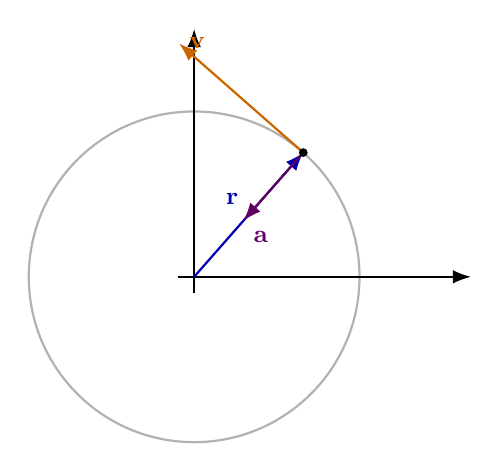
\begin{tikzpicture}[>=Latex, thick, scale=1.05, trig format=rad]
  \def\R{2.0}
  \def\ang{0.85}
  \coordinate (O) at (0,0);
  \coordinate (P) at ({\R*cos(\ang)},{\R*sin(\ang)});
  \draw[gray!60] (O) circle (\R);
  \draw[->] (-0.2,0) -- (\R+1.35,0);
  \draw[->] (0,-0.2) -- (0,\R+1.0);
  \draw[blue!70!black,->] (O) -- (P) node[midway, above left, font=\small]{$\mathbf{r}$};
  \draw[orange!80!black,->] (P) -- ($ (P) + ({-\R*sin(\ang)},{\R*cos(\ang)}) $)
    node[right, font=\small]{$\mathbf{v}$};
  \draw[violet!75!black,->] (P) -- ($ (P) + ({-0.55*\R*cos(\ang)},{-0.55*\R*sin(\ang)}) $)
    node[below right, font=\small]{$\mathbf{a}$};
  \fill (P) circle (1.5pt);
\end{tikzpicture}
\end{center}

\resultbox{With \(\mathbf{v}\) and \(\mathbf{a}\) as above, \(\mathbf{v}\cdot\mathbf{a}=0\), so velocity and acceleration are orthogonal. For \(\mathbf{r}=R(\cos\omega t,\sin\omega t)\), also \(\mathbf{r}\cdot\mathbf{v}=0\).}

\examplebox{At \(\omega t=\pi/4\): \(\mathbf{v}\propto(-1,1)\), \(\mathbf{a}\propto(-1,-1)\); their dot product is zero.}

\end{document}
